\documentclass[tikz]{standalone}
\usepackage{amsmath}
\usepackage{amssymb}
\usepackage{amsfonts}
\usepackage{tikz}
\usetikzlibrary{circuits.logic.US}

\thispagestyle{empty}
\begin{document}
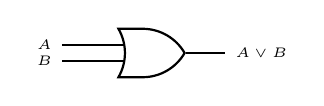
\begin{tikzpicture}[thick, circuit logic US]
% Input A at (0,0)
\node at (0,0) (A) {\tiny $A$};
\node at (0.0,-0.205) (B) {\tiny $B$};

% Place AND gate so that input 1 aligns with A at (0,0)
\node[or gate, anchor=input 1] at (1,0) (and1) {};

% Wires from A and B
\draw (A) --  ++(1.015,0) |- (and1.input 1);
\draw (B) -- ++(0.25,0) -- ++(0.715,0) |- (and1.input 2); % Very hack-ish, sorry :(

% Output
\draw (and1.output) -- ++(0.5,0) node[right] {\tiny $A \lor B$};
\end{tikzpicture}

\end{document}
